\subsection{Radanpassung}\label{cap:methoden_radanpassung}
\begin{figure}[ht]
  \begin{center}
    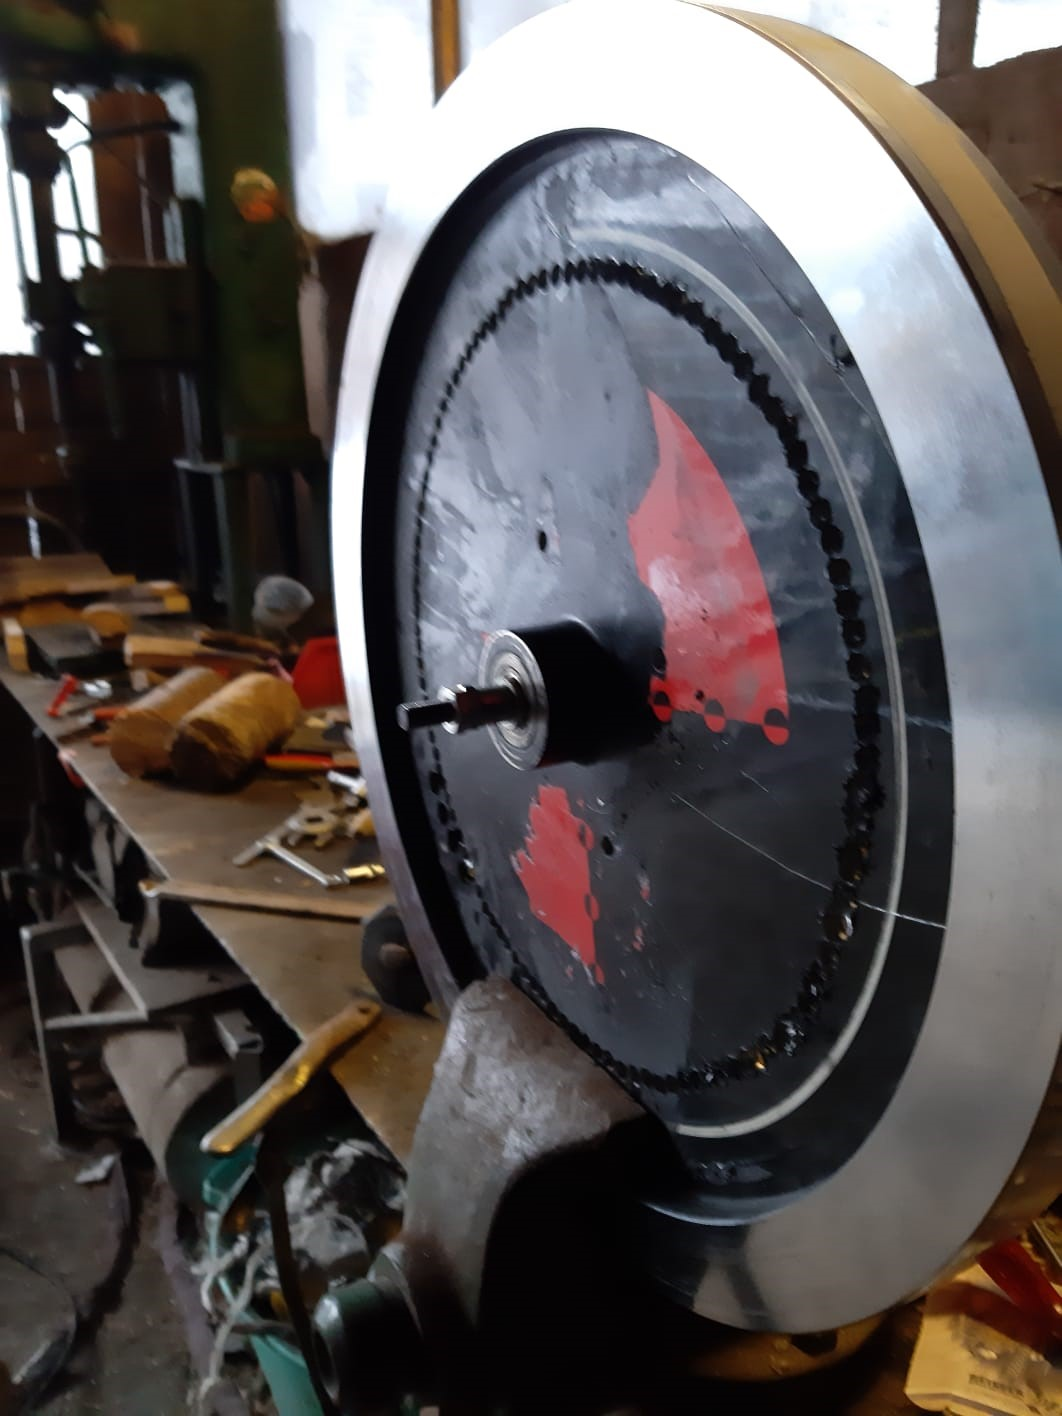
\includegraphics[width=8cm]{assets/images/rad}
  \end{center}
  \vspace{-3ex}
  \caption{Radanpassung durch Bohrungen}
  \label{fig:radanpassung_bild}
\end{figure}
Nach ersten Bremsversuchen wurde klar, welche hohe kinetische Energie in einem schweren Rad stecken kann. Das massive Rad verzögerte nicht erwartungsgemäss, aufgrund der nicht beachteten Trägheit.
\newpara
Da der maximale Wert des Stromflusses innerhalb der Spulen bereits erreicht wurde, musste eine andere Lösung her. Um eine stärkere Verzögerung zu erzielen, wurde das Gewicht, des zu Beginn vorhandene Schwungrad reduziert. 
\newpara
Der Radius des grösseren Schwungrades wurde auf den Durchmesser der anderen zwei Scheiben angepasst. Dieser Vorgang erfolgte durch Bohrungen entlang dem Umkreis der Bremsscheibe (Siehe Abbildung \ref{fig:radanpassung_bild}). Somit verlor das gesamte Rad ungefähr 60\% an Masse.
\newpara
Durch diesen Gewichtsverlust wird eine deutlich stärkere Verzögerung erwartet.